% This TeX document is part of the manual of the GNU Astronomy
% Utilities (Gnuastro). A Makefile is also distributed which allows
% you to compile this TeX file in the desired manner.
%
% Original author:
%     Mohammad Akhlaghi <mohammad@akhlaghi.org>
% Contributing author(s):
% Copyright (C) 2016-2023 Free Software Foundation, Inc.
%
% Gnuastro is free software: you can redistribute it and/or modify it
% under the terms of the GNU General Public License as published by
% the Free Software Foundation, either version 3 of the License, or
% (at your option) any later version.
%
% Gnuastro is distributed in the hope that it will be useful, but
% WITHOUT ANY WARRANTY; without even the implied warranty of
% MERCHANTABILITY or FITNESS FOR A PARTICULAR PURPOSE.  See the GNU
% General Public License for more details.
%
% You should have received a copy of the GNU General Public License
% along with Gnuastro. If not, see <http://www.gnu.org/licenses/>.

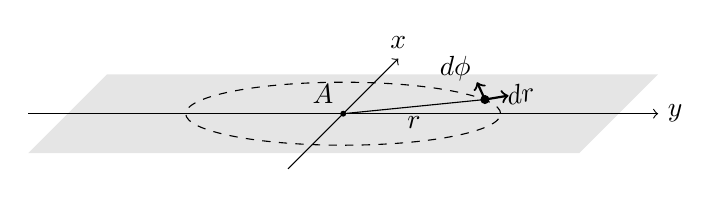
\begin{tikzpicture}

  \fill[fill=black!10!white]
  (-2.5,0.5) -- ++(7,0) -- ++(-1,-1) -- ++(-7,0) -- cycle;

  \filldraw (0.5,0) circle (0.03);
  \draw (0.5,0) node[anchor=south east]{$A$};
  \draw[dashed] (0.5,0) ellipse (2 and 0.4);
  \draw (0.5,0) -- node[anchor=north]{$r$}(2.3,0.18);
  \filldraw (2.3,0.18) circle (0.05);
  \draw[->, thick]
  (2.3,0.18) -- node[anchor=west, rotate=10]{$dr$}(2.6,0.23);
  \draw[->, thick]
  (2.3,0.18) -- node[anchor=south east]{$d\phi$}(2.2,0.4);
  \draw[<-, thin] (1.2,0.7) -- (-0.2,-0.7); %along y=x-0.5
  \draw[->, thin] (-3.5,0) -- (4.5,0);
  \draw (1.2,0.7) node[anchor=south]{$x$};
  \draw (4.5,0) node[anchor=west]{$y$};

\end{tikzpicture}
